\documentclass[NEMO_book]{subfiles}
\begin{document}
% ================================================================
% Chapter 1 ——— Ocean Tracers (TRA)
% ================================================================
\chapter{Ocean Tracers (TRA)}
\label{TRA}
\minitoc

% missing/update 
% traqsr: need to coordinate with SBC module

%STEVEN :  is the use of the word "positive" to describe a scheme enough, or should it be "positive definite"? I added a comment to this effect on some instances of this below

%\newpage
\vspace{2.cm}
%$\ $\newline    % force a new ligne

Using the representation described in Chap.~\ref{DOM}, several semi-discrete 
space forms of the tracer equations are available depending on the vertical 
coordinate used and on the physics used. In all the equations presented 
here, the masking has been omitted for simplicity. One must be aware that 
all the quantities are masked fields and that each time a mean or difference 
operator is used, the resulting field is multiplied by a mask.

The two active tracers are potential temperature and salinity. Their prognostic 
equations can be summarized as follows:
\begin{equation*}
\text{NXT} = \text{ADV}+\text{LDF}+\text{ZDF}+\text{SBC}
                   \ (+\text{QSR})\ (+\text{BBC})\ (+\text{BBL})\ (+\text{DMP})
\end{equation*}

NXT stands for next, referring to the time-stepping. From left to right, the terms 
on the rhs of the tracer equations are the advection (ADV), the lateral diffusion 
(LDF), the vertical diffusion (ZDF), the contributions from the external forcings 
(SBC: Surface Boundary Condition, QSR: penetrative Solar Radiation, and BBC: 
Bottom Boundary Condition), the contribution from the bottom boundary Layer 
(BBL) parametrisation, and an internal damping (DMP) term. The terms QSR, 
BBC, BBL and DMP are optional. The external forcings and parameterisations 
require complex inputs and complex calculations ($e.g.$ bulk formulae, estimation 
of mixing coefficients) that are carried out in the SBC, LDF and ZDF modules and 
described in chapters \S\ref{SBC}, \S\ref{LDF} and  \S\ref{ZDF}, respectively. 
Note that \mdl{tranpc}, the non-penetrative convection module, although 
located in the NEMO/OPA/TRA directory as it directly modifies the tracer fields, 
is described with the model vertical physics (ZDF) together with other available 
parameterization of convection.

In the present chapter we also describe the diagnostic equations used to compute 
the sea-water properties (density, Brunt-V\"{a}is\"{a}l\"{a} frequency, specific heat and 
freezing point with associated modules \mdl{eosbn2} and \mdl{phycst}).

The different options available to the user are managed by namelist logicals or 
CPP keys. For each equation term \textit{ttt}, the namelist logicals are \textit{ln\_trattt\_xxx}, 
where \textit{xxx} is a 3 or 4 letter acronym corresponding to each optional scheme. 
The CPP key (when it exists) is \textbf{key\_trattt}. The equivalent code can be 
found in the \textit{trattt} or \textit{trattt\_xxx} module, in the NEMO/OPA/TRA directory.

The user has the option of extracting each tendency term on the RHS of the tracer 
equation for output (\np{ln\_tra\_trd} or \np{ln\_tra\_mxl}~=~true), as described in Chap.~\ref{DIA}.

$\ $\newline    % force a new ligne
% ================================================================
% Tracer Advection
% ================================================================
\section  [Tracer Advection (\textit{traadv})]
		{Tracer Advection (\mdl{traadv})}
\label{TRA_adv}
%------------------------------------------namtra_adv-----------------------------------------------------
\namdisplay{namtra_adv}
%-------------------------------------------------------------------------------------------------------------

The advection tendency of a tracer in flux form is the divergence of the advective 
fluxes. Its discrete expression is given by :
\begin{equation} \label{Eq_tra_adv}
ADV_\tau =-\frac{1}{b_t} \left( 
\;\delta _i \left[ e_{2u}\,e_{3u} \;  u\; \tau _u  \right]
+\delta _j \left[ e_{1v}\,e_{3v}  \;  v\; \tau _v  \right] \; \right)
-\frac{1}{e_{3t}} \;\delta _k \left[ w\; \tau _w \right]
\end{equation}
where $\tau$ is either T or S, and $b_t= e_{1t}\,e_{2t}\,e_{3t}$ is the volume of $T$-cells. 
The flux form in \eqref{Eq_tra_adv} 
implicitly requires the use of the continuity equation. Indeed, it is obtained
by using the following equality : $\nabla \cdot \left( \vect{U}\,T \right)=\vect{U} \cdot \nabla T$ 
which results from the use of the continuity equation, $\nabla \cdot \vect{U}=0$ or 
$ \partial _t e_3 + e_3\;\nabla \cdot \vect{U}=0$ in constant volume or variable volume case, respectively. 
Therefore it is of paramount importance to design the discrete analogue of the 
advection tendency so that it is consistent with the continuity equation in order to 
enforce the conservation properties of the continuous equations. In other words, 
by replacing $\tau$ by the number 1 in (\ref{Eq_tra_adv}) we recover the discrete form of 
the continuity equation which is used to calculate the vertical velocity.
%>>>>>>>>>>>>>>>>>>>>>>>>>>>>
\begin{figure}[!t] 	 \begin{center}
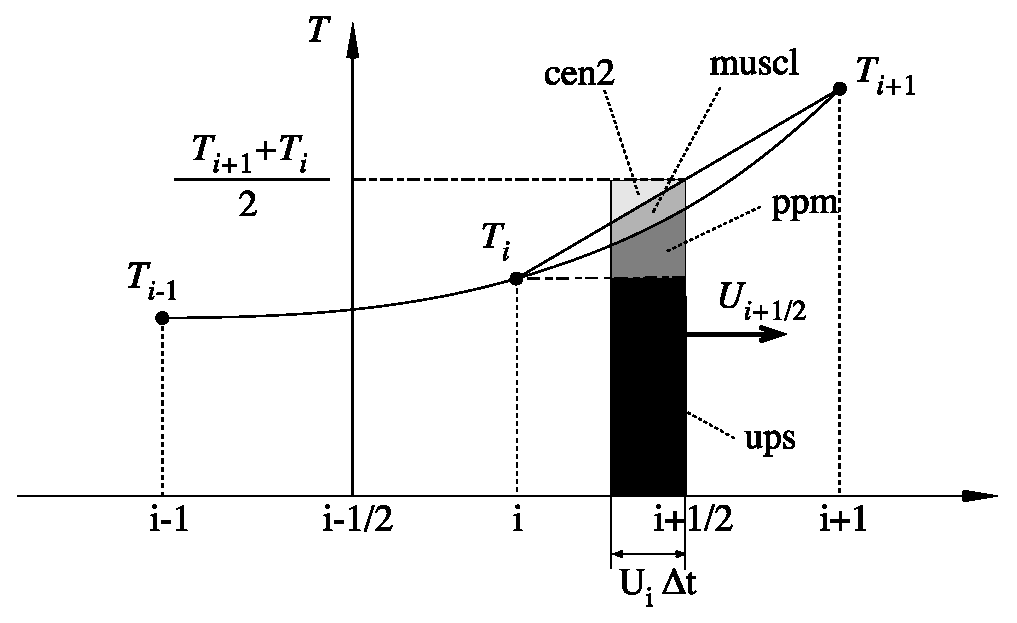
\includegraphics[width=0.9\textwidth]{Fig_adv_scheme}
\caption{	\label{Fig_adv_scheme} 
Schematic representation of some ways used to evaluate the tracer value 
at $u$-point and the amount of tracer exchanged between two neighbouring grid 
points. Upsteam biased scheme (ups): the upstream value is used and the black 
area is exchanged. Piecewise parabolic method (ppm): a parabolic interpolation 
is used and the black and dark grey areas are exchanged. Monotonic upstream 
scheme for conservative laws (muscl):  a parabolic interpolation is used and black, 
dark grey and grey areas are exchanged. Second order scheme (cen2): the mean 
value is used and black, dark grey, grey and light grey areas are exchanged. Note 
that this illustration does not include the flux limiter used in ppm and muscl schemes.}
\end{center}   \end{figure}
%>>>>>>>>>>>>>>>>>>>>>>>>>>>>

The key difference between the advection schemes available in \NEMO is the choice 
made in space and time interpolation to define the value of the tracer at the 
velocity points (Fig.~\ref{Fig_adv_scheme}). 

Along solid lateral and bottom boundaries a zero tracer flux is automatically 
specified, since the normal velocity is zero there. At the sea surface the 
boundary condition depends on the type of sea surface chosen: 
\begin{description}
\item [linear free surface:] the first level thickness is constant in time: 
the vertical boundary condition is applied at the fixed surface $z=0$ 
rather than on the moving surface $z=\eta$. There is a non-zero advective 
flux which is set for all advection schemes as 
$\left. {\tau _w } \right|_{k=1/2} =T_{k=1} $, $i.e.$ 
the product of surface velocity (at $z=0$) by the first level tracer value.
\item [non-linear free surface:] (\key{vvl} is defined) 
convergence/divergence in the first ocean level moves the free surface 
up/down. There is no tracer advection through it so that the advective 
fluxes through the surface are also zero 
\end{description}
In all cases, this boundary condition retains local conservation of tracer. 
Global conservation is obtained in non-linear free surface case, 
but \textit{not} in the linear free surface case. Nevertheless, in the latter case, 
it is achieved to a good approximation since the non-conservative 
term is the product of the time derivative of the tracer and the free surface 
height, two quantities that are not correlated (see \S\ref{PE_free_surface}, 
and also \citet{Roullet_Madec_JGR00,Griffies_al_MWR01,Campin2004}).

The velocity field that appears in (\ref{Eq_tra_adv}) and (\ref{Eq_tra_adv_zco}) 
is the centred (\textit{now}) \textit{effective} ocean velocity, $i.e.$ the \textit{eulerian} velocity
(see Chap.~\ref{DYN}) plus the eddy induced velocity (\textit{eiv}) 
and/or the mixed layer eddy induced velocity (\textit{eiv})
when those parameterisations are used (see Chap.~\ref{LDF}).

The choice of an advection scheme is made in the \textit{\ngn{nam\_traadv}} namelist, by 
setting to \textit{true} one and only one of the logicals \textit{ln\_traadv\_xxx}. The 
corresponding code can be found in the \textit{traadv\_xxx.F90} module, where 
\textit{xxx} is a 3 or 4 letter acronym corresponding to each scheme. Details 
of the advection schemes are given below. The choice of an advection scheme 
is a complex matter which depends on the model physics, model resolution, 
type of tracer, as well as the issue of numerical cost. 

Note that 
(1) cen2 and TVD schemes require an explicit diffusion 
operator while the other schemes are diffusive enough so that they do not 
require additional diffusion ; 
(2) cen2, MUSCL2, and UBS are not \textit{positive} schemes
\footnote{negative values can appear in an initially strictly positive tracer field 
which is advected}
, implying that false extrema are permitted. Their use is not recommended on passive tracers ; 
(3) It is recommended that the same advection-diffusion scheme is 
used on both active and passive tracers. Indeed, if a source or sink of a 
passive tracer depends on an active one, the difference of treatment of 
active and passive tracers can create very nice-looking frontal structures 
that are pure numerical artefacts. Nevertheless, most of our users set a different 
treatment on passive and active tracers, that's the reason why this possibility 
is offered. We strongly suggest them to perform a sensitivity experiment 
using a same treatment to assess the robustness of their results.

% -------------------------------------------------------------------------------------------------------------
%        2nd order centred scheme  
% -------------------------------------------------------------------------------------------------------------
\subsection   [$2^{nd}$ order centred scheme (cen2) (\np{ln\_traadv\_cen2})]
			{$2^{nd}$ order centred scheme (cen2) (\np{ln\_traadv\_cen2}=true)}
\label{TRA_adv_cen2}

In the centred second order formulation, the tracer at velocity points is 
evaluated as the mean of the two neighbouring $T$-point values. 
For example, in the $i$-direction :
\begin{equation} \label{Eq_tra_adv_cen2}
\tau _u^{cen2} =\overline T ^{i+1/2}
\end{equation}

The scheme is non diffusive ($i.e.$ it conserves the tracer variance, $\tau^2)$ 
but dispersive ($i.e.$ it may create false extrema). It is therefore notoriously 
noisy and must be used in conjunction with an explicit diffusion operator to 
produce a sensible solution. The associated time-stepping is performed using 
a leapfrog scheme in conjunction with an Asselin time-filter, so $T$ in 
(\ref{Eq_tra_adv_cen2}) is the \textit{now} tracer value. The centered second 
order advection is computed in the \mdl{traadv\_cen2} module. In this module,
it is advantageous to combine the \textit{cen2} scheme with an upstream scheme
in specific areas which require a strong diffusion in order to avoid the generation 
of false extrema. These areas are the vicinity of large river mouths, some straits 
with coarse resolution, and the vicinity of ice cover area ($i.e.$ when the ocean 
temperature is close to the freezing point).
This combined scheme has been included for specific grid points in the ORCA2 
configuration only. This is an obsolescent feature as the recommended 
advection scheme for the ORCA configuration is TVD (see  \S\ref{TRA_adv_tvd}).

Note that using the cen2 scheme, the overall tracer advection is of second 
order accuracy since both (\ref{Eq_tra_adv}) and (\ref{Eq_tra_adv_cen2}) 
have this order of accuracy. \gmcomment{Note also that ... blah, blah}


% -------------------------------------------------------------------------------------------------------------
%        TVD scheme  
% -------------------------------------------------------------------------------------------------------------
\subsection   [Total Variance Dissipation scheme (TVD) (\np{ln\_traadv\_tvd})]
			{Total Variance Dissipation scheme (TVD) (\np{ln\_traadv\_tvd}=true)}
\label{TRA_adv_tvd}

In the Total Variance Dissipation (TVD) formulation, the tracer at velocity 
points is evaluated using a combination of an upstream and a centred scheme. 
For example, in the $i$-direction :
\begin{equation} \label{Eq_tra_adv_tvd}
\begin{split}
\tau _u^{ups}&= \begin{cases}
 					T_{i+1} 	& \text{if $\ u_{i+1/2} <     0$} \hfill \\
 					T_i   		& \text{if $\ u_{i+1/2} \geq 0$} \hfill \\
				  \end{cases}     \\
\\
\tau _u^{tvd}&=\tau _u^{ups} +c_u \;\left( {\tau _u^{cen2} -\tau _u^{ups} } \right)
\end{split}
\end{equation}
where $c_u$ is a flux limiter function taking values between 0 and 1. 
There exist many ways to define $c_u$, each corresponding to a different 
total variance decreasing scheme. The one chosen in \NEMO is described in 
\citet{Zalesak_JCP79}. $c_u$ only departs from $1$ when the advective term 
produces a local extremum in the tracer field. The resulting scheme is quite 
expensive but \emph{positive}. It can be used on both active and passive tracers. 
This scheme is tested and compared with MUSCL and the MPDATA scheme in 
\citet{Levy_al_GRL01}; note that in this paper it is referred to as "FCT" (Flux corrected 
transport) rather than TVD. The TVD scheme is implemented in the \mdl{traadv\_tvd} module.

For stability reasons (see \S\ref{STP}),
$\tau _u^{cen2}$ is evaluated  in (\ref{Eq_tra_adv_tvd}) using the \textit{now} tracer while $\tau _u^{ups}$ 
is evaluated using the \textit{before} tracer. In other words, the advective part of 
the scheme is time stepped with a leap-frog scheme while a forward scheme is 
used for the diffusive part. 

An additional option has been added controlled by \np{ln\_traadv\_tvd\_zts}. 
By setting this logical to true, a TVD scheme is used on both horizontal and vertical direction, 
but on the latter, a split-explicit time stepping is used, with 5 sub-timesteps. 
This option can be useful when the value of the timestep is limited by vertical advection \citep{Lemarie_OM2015}. 
Note that in this case, a similar split-explicit time stepping should be used on 
vertical advection of momentum to ensure a better stability (see \np{ln\_dynzad\_zts} in \S\ref{DYN_zad}).


% -------------------------------------------------------------------------------------------------------------
%        MUSCL scheme  
% -------------------------------------------------------------------------------------------------------------
\subsection[MUSCL scheme  (\np{ln\_traadv\_muscl})]
	{Monotone Upstream Scheme for Conservative Laws (MUSCL) (\np{ln\_traadv\_muscl}=T)}
\label{TRA_adv_muscl}

The Monotone Upstream Scheme for Conservative Laws (MUSCL) has been 
implemented by \citet{Levy_al_GRL01}. In its formulation, the tracer at velocity points 
is evaluated assuming a linear tracer variation between two $T$-points 
(Fig.\ref{Fig_adv_scheme}). For example, in the $i$-direction :
\begin{equation} \label{Eq_tra_adv_muscl}
   \tau _u^{mus} = \left\{      \begin{aligned}
         &\tau _i  &+ \frac{1}{2} \;\left( 1-\frac{u_{i+1/2} \;\rdt}{e_{1u}} \right)
         &\ \widetilde{\partial _i \tau}  & \quad \text{if }\;u_{i+1/2} \geqslant 0      \\
         &\tau _{i+1/2} &+\frac{1}{2}\;\left( 1+\frac{u_{i+1/2} \;\rdt}{e_{1u} } \right)
         &\ \widetilde{\partial_{i+1/2} \tau } & \text{if }\;u_{i+1/2} <0
   \end{aligned}    \right.
\end{equation}
where $\widetilde{\partial _i \tau}$ is the slope of the tracer on which a limitation 
is imposed to ensure the \textit{positive} character of the scheme.

The time stepping is performed using a forward scheme, that is the \textit{before} 
tracer field is used to evaluate $\tau _u^{mus}$.

For an ocean grid point adjacent to land and where the ocean velocity is 
directed toward land, two choices are available: an upstream flux (\np{ln\_traadv\_muscl}=true) 
or a second order flux (\np{ln\_traadv\_muscl2}=true). 
Note that the latter choice does not ensure the \textit{positive} character of the scheme. 
Only the former can be used on both active and passive tracers. 
The two MUSCL schemes are implemented in the \mdl{traadv\_tvd} and \mdl{traadv\_tvd2} modules.

Note that when using np{ln\_traadv\_msc\_ups}~=~true in addition to \np{ln\_traadv\_muscl}=true, 
the MUSCL fluxes are replaced by upstream fluxes in vicinity of river mouths.

% -------------------------------------------------------------------------------------------------------------
%        UBS scheme  
% -------------------------------------------------------------------------------------------------------------
\subsection   [Upstream-Biased Scheme (UBS) (\np{ln\_traadv\_ubs})]
			{Upstream-Biased Scheme (UBS) (\np{ln\_traadv\_ubs}=true)}
\label{TRA_adv_ubs}

The UBS advection scheme is an upstream-biased third order scheme based on 
an upstream-biased parabolic interpolation. It is also known as the Cell 
Averaged QUICK scheme (Quadratic Upstream Interpolation for Convective 
Kinematics). For example, in the $i$-direction :
\begin{equation} \label{Eq_tra_adv_ubs}
   \tau _u^{ubs} =\overline T ^{i+1/2}-\;\frac{1}{6} \left\{      
   \begin{aligned}
         &\tau"_i        	& \quad \text{if }\ u_{i+1/2} \geqslant 0      \\
         &\tau"_{i+1}	& \quad \text{if }\ u_{i+1/2}       <       0
   \end{aligned}    \right.
\end{equation}
where $\tau "_i =\delta _i \left[ {\delta _{i+1/2} \left[ \tau \right]} \right]$.

This results in a dissipatively dominant (i.e. hyper-diffusive) truncation 
error \citep{Shchepetkin_McWilliams_OM05}. The overall performance of the advection 
scheme is similar to that reported in \cite{Farrow1995}. 
It is a relatively good compromise between accuracy and smoothness. 
It is not a \emph{positive} scheme, meaning that false extrema are permitted, 
but the amplitude of such are significantly reduced over the centred second 
order method. Nevertheless it is not recommended that it should be applied 
to a passive tracer that requires positivity. 

The intrinsic diffusion of UBS makes its use risky in the vertical direction 
where the control of artificial diapycnal fluxes is of paramount importance. 
Therefore the vertical flux is evaluated using the TVD scheme when 
\np{ln\_traadv\_ubs}=true.

For stability reasons  (see \S\ref{STP}),
the first term  in \eqref{Eq_tra_adv_ubs} (which corresponds to a second order centred scheme) 
is evaluated using the \textit{now} tracer (centred in time) while the 
second term (which is the diffusive part of the scheme), is 
evaluated using the \textit{before} tracer (forward in time). 
This choice is discussed by \citet{Webb_al_JAOT98} in the context of the 
QUICK advection scheme. UBS and QUICK schemes only differ 
by one coefficient. Replacing 1/6 with 1/8 in \eqref{Eq_tra_adv_ubs} 
leads to the QUICK advection scheme \citep{Webb_al_JAOT98}. 
This option is not available through a namelist parameter, since the 
1/6 coefficient is hard coded. Nevertheless it is quite easy to make the 
substitution in the \mdl{traadv\_ubs} module and obtain a QUICK scheme.

Four different options are possible for the vertical 
component used in the UBS scheme. $\tau _w^{ubs}$ can be evaluated 
using either \textit{(a)} a centred $2^{nd}$ order scheme, or  \textit{(b)} 
a TVD scheme, or  \textit{(c)} an interpolation based on conservative 
parabolic splines following the \citet{Shchepetkin_McWilliams_OM05} 
implementation of UBS in ROMS, or  \textit{(d)} a UBS. The $3^{rd}$ case 
has dispersion properties similar to an eighth-order accurate conventional scheme.
The current reference version uses method b)

Note that :

(1) When a high vertical resolution $O(1m)$ is used, the model stability can 
be controlled by vertical advection (not vertical diffusion which is usually 
solved using an implicit scheme). Computer time can be saved by using a 
time-splitting technique on vertical advection. Such a technique has been 
implemented and validated in ORCA05 with 301 levels. It is not available 
in the current reference version. 

(2) It is straightforward to rewrite \eqref{Eq_tra_adv_ubs} as follows:
\begin{equation} \label{Eq_traadv_ubs2}
\tau _u^{ubs} = \tau _u^{cen4} + \frac{1}{12} \left\{	 
   \begin{aligned}
	& + \tau"_i			& \quad \text{if }\ u_{i+1/2} \geqslant 0 \\
	&  - \tau"_{i+1}		& \quad \text{if }\ u_{i+1/2}       <       0
   \end{aligned}    \right.
\end{equation}
or equivalently 
\begin{equation} \label{Eq_traadv_ubs2b}
u_{i+1/2} \ \tau _u^{ubs} 
=u_{i+1/2} \ \overline{ T - \frac{1}{6}\,\delta _i\left[ \delta_{i+1/2}[T] \,\right] }^{\,i+1/2}
- \frac{1}{2} |u|_{i+1/2} \;\frac{1}{6} \;\delta_{i+1/2}[\tau"_i]
\end{equation}

\eqref{Eq_traadv_ubs2} has several advantages. Firstly, it clearly reveals 
that the UBS scheme is based on the fourth order scheme to which an 
upstream-biased diffusion term is added. Secondly, this emphasises that the 
$4^{th}$ order part (as well as the $2^{nd}$ order part as stated above) has 
to be evaluated at the \emph{now} time step using \eqref{Eq_tra_adv_ubs}. 
Thirdly, the diffusion term is in fact a biharmonic operator with an eddy 
coefficient which is simply proportional to the velocity:
 $A_u^{lm}= - \frac{1}{12}\,{e_{1u}}^3\,|u|$. Note that NEMO v3.4 still uses 
 \eqref{Eq_tra_adv_ubs}, not \eqref{Eq_traadv_ubs2}.
 %%%
 \gmcomment{the change in UBS scheme has to be done}
 %%%

% -------------------------------------------------------------------------------------------------------------
%        QCK scheme  
% -------------------------------------------------------------------------------------------------------------
\subsection   [QUICKEST scheme (QCK) (\np{ln\_traadv\_qck})]
			{QUICKEST scheme (QCK) (\np{ln\_traadv\_qck}=true)}
\label{TRA_adv_qck}

The Quadratic Upstream Interpolation for Convective Kinematics with 
Estimated Streaming Terms (QUICKEST) scheme proposed by \citet{Leonard1979} 
is the third order Godunov scheme. It is associated with the ULTIMATE QUICKEST 
limiter \citep{Leonard1991}. It has been implemented in NEMO by G. Reffray 
(MERCATOR-ocean) and can be found in the \mdl{traadv\_qck} module.
The resulting scheme is quite expensive but \emph{positive}. 
It can be used on both active and passive tracers. 
However, the intrinsic diffusion of QCK makes its use risky in the vertical 
direction where the control of artificial diapycnal fluxes is of paramount importance. 
Therefore the vertical flux is evaluated using the CEN2 scheme. 
This no longer guarantees the positivity of the scheme. The use of TVD in the vertical 
direction (as for the UBS case) should be implemented to restore this property.


% ================================================================
% Tracer Lateral Diffusion
% ================================================================
\section  [Tracer Lateral Diffusion (\textit{traldf})]
		{Tracer Lateral Diffusion (\mdl{traldf})}
\label{TRA_ldf}
%-----------------------------------------nam_traldf------------------------------------------------------
\namdisplay{namtra_ldf}
%-------------------------------------------------------------------------------------------------------------
 
Options are defined through the  \ngn{namtra\_ldf} namelist variables.
The options available for lateral diffusion are a laplacian (rotated or not) 
or a biharmonic operator, the latter being more scale-selective (more 
diffusive at small scales). The specification of eddy diffusivity 
coefficients (either constant or variable in space and time) as well as the 
computation of the slope along which the operators act, are performed in the 
\mdl{ldftra} and \mdl{ldfslp} modules, respectively. This is described in Chap.~\ref{LDF}. 
The lateral diffusion of tracers is evaluated using a forward scheme, 
$i.e.$ the tracers appearing in its expression are the \textit{before} tracers in time, 
except for the pure vertical component that appears when a rotation tensor 
is used. This latter term is solved implicitly together with the 
vertical diffusion term (see \S\ref{STP}).

% -------------------------------------------------------------------------------------------------------------
%        Iso-level laplacian operator
% -------------------------------------------------------------------------------------------------------------
\subsection   [Iso-level laplacian operator (lap) (\np{ln\_traldf\_lap})]
			{Iso-level laplacian operator (lap) (\np{ln\_traldf\_lap}=true) }
\label{TRA_ldf_lap}

A laplacian diffusion operator ($i.e.$ a harmonic operator) acting along the model 
surfaces is given by: 
\begin{equation} \label{Eq_tra_ldf_lap}
D_T^{lT} =\frac{1}{b_t} \left( \;
   \delta _{i}\left[ A_u^{lT} \; \frac{e_{2u}\,e_{3u}}{e_{1u}} \;\delta _{i+1/2} [T] \right] 
+ \delta _{j}\left[ A_v^{lT} \;  \frac{e_{1v}\,e_{3v}}{e_{2v}} \;\delta _{j+1/2} [T] \right]  \;\right)
\end{equation}
where  $b_t$=$e_{1t}\,e_{2t}\,e_{3t}$  is the volume of $T$-cells. 
It is implemented in the \mdl{traadv\_lap} module.

This lateral operator is computed in \mdl{traldf\_lap}. It is a \emph{horizontal} 
operator ($i.e.$ acting along geopotential surfaces) in the $z$-coordinate with 
or without partial steps, but is simply an iso-level operator in the $s$-coordinate. 
It is thus used when, in addition to \np{ln\_traldf\_lap}=true, we have 
\np{ln\_traldf\_level}=true or \np{ln\_traldf\_hor}=\np{ln\_zco}=true. 
In both cases, it significantly contributes to diapycnal mixing. 
It is therefore not recommended.

Note that in the partial step $z$-coordinate (\np{ln\_zps}=true), tracers in horizontally 
adjacent cells are located at different depths in the vicinity of the bottom. 
In this case, horizontal derivatives in (\ref{Eq_tra_ldf_lap}) at the bottom level 
require a specific treatment. They are calculated in the \mdl{zpshde} module, 
described in \S\ref{TRA_zpshde}.

% -------------------------------------------------------------------------------------------------------------
%        Rotated laplacian operator
% -------------------------------------------------------------------------------------------------------------
\subsection   [Rotated laplacian operator (iso) (\np{ln\_traldf\_lap})]
			{Rotated laplacian operator (iso) (\np{ln\_traldf\_lap}=true)}
\label{TRA_ldf_iso}

If the Griffies trad scheme is not employed
(\np{ln\_traldf\_grif}=true; see App.\ref{sec:triad}) the general form of the second order lateral tracer subgrid scale physics 
(\ref{Eq_PE_zdf}) takes the following semi-discrete space form in $z$- and 
$s$-coordinates:
\begin{equation} \label{Eq_tra_ldf_iso}
\begin{split}
 D_T^{lT} = \frac{1}{b_t}   & \left\{   \,\;\delta_i \left[   A_u^{lT}  \left( 
	  \frac{e_{2u}\,e_{3u}}{e_{1u}} \,\delta_{i+1/2}[T]
	- e_{2u}\;r_{1u} \,\overline{\overline{ \delta_{k+1/2}[T] }}^{\,i+1/2,k}
                                                     \right)   \right]   \right.    \\ 
&             +\delta_j \left[ A_v^{lT} \left( 
          \frac{e_{1v}\,e_{3v}}{e_{2v}}  \,\delta_{j+1/2} [T] 
        - e_{1v}\,r_{2v} \,\overline{\overline{ \delta_{k+1/2} [T] }}^{\,j+1/2,k} 
                                                    \right)   \right]                 \\ 
& +\delta_k \left[ A_w^{lT} \left( 
       -\;e_{2w}\,r_{1w} \,\overline{\overline{ \delta_{i+1/2} [T] }}^{\,i,k+1/2}
                                                    \right.   \right.                 \\ 
& \qquad \qquad \quad 
        - e_{1w}\,r_{2w} \,\overline{\overline{ \delta_{j+1/2} [T] }}^{\,j,k+1/2}     \\
& \left. {\left. {   \qquad \qquad \ \ \ \left. {
        +\;\frac{e_{1w}\,e_{2w}}{e_{3w}} \,\left( r_{1w}^2 + r_{2w}^2 \right)
           \,\delta_{k+1/2} [T] } \right) } \right] \quad } \right\} 
 \end{split}
 \end{equation}
where $b_t$=$e_{1t}\,e_{2t}\,e_{3t}$  is the volume of $T$-cells, 
$r_1$ and $r_2$ are the slopes between the surface of computation 
($z$- or $s$-surfaces) and the surface along which the diffusion operator 
acts ($i.e.$ horizontal or iso-neutral surfaces).  It is thus used when, 
in addition to \np{ln\_traldf\_lap}= true, we have \np{ln\_traldf\_iso}=true, 
or both \np{ln\_traldf\_hor}=true and \np{ln\_zco}=true. The way these 
slopes are evaluated is given in \S\ref{LDF_slp}. At the surface, bottom 
and lateral boundaries, the turbulent fluxes of heat and salt are set to zero 
using the mask technique (see \S\ref{LBC_coast}). 

The operator in \eqref{Eq_tra_ldf_iso} involves both lateral and vertical 
derivatives. For numerical stability, the vertical second derivative must 
be solved using the same implicit time scheme as that used in the vertical 
physics (see \S\ref{TRA_zdf}). For computer efficiency reasons, this term 
is not computed in the \mdl{traldf\_iso} module, but in the \mdl{trazdf} module 
where, if iso-neutral mixing is used, the vertical mixing coefficient is simply 
increased by $\frac{e_{1w}\,e_{2w} }{e_{3w} }\ \left( {r_{1w} ^2+r_{2w} ^2} \right)$. 

This formulation conserves the tracer but does not ensure the decrease 
of the tracer variance. Nevertheless the treatment performed on the slopes 
(see \S\ref{LDF}) allows the model to run safely without any additional 
background horizontal diffusion \citep{Guilyardi_al_CD01}. An alternative scheme 
developed by \cite{Griffies_al_JPO98} which ensures tracer variance decreases 
is also available in \NEMO (\np{ln\_traldf\_grif}=true). A complete description of 
the algorithm is given in App.\ref{sec:triad}.

Note that in the partial step $z$-coordinate (\np{ln\_zps}=true), the horizontal 
derivatives at the bottom level in \eqref{Eq_tra_ldf_iso} require a specific 
treatment. They are calculated in module zpshde, described in \S\ref{TRA_zpshde}.

% -------------------------------------------------------------------------------------------------------------
%        Iso-level bilaplacian operator
% -------------------------------------------------------------------------------------------------------------
\subsection   [Iso-level bilaplacian operator (bilap) (\np{ln\_traldf\_bilap})]
			{Iso-level bilaplacian operator (bilap) (\np{ln\_traldf\_bilap}=true)}
\label{TRA_ldf_bilap}

The lateral fourth order bilaplacian operator on tracers is obtained by 
applying (\ref{Eq_tra_ldf_lap}) twice. The operator requires an additional assumption 
on boundary conditions: both first and third derivative terms normal to the 
coast are set to zero. It is used when, in addition to \np{ln\_traldf\_bilap}=true, 
we have \np{ln\_traldf\_level}=true, or both \np{ln\_traldf\_hor}=true and 
\np{ln\_zco}=false. In both cases, it can contribute diapycnal mixing, 
although less than in the laplacian case. It is therefore not recommended.

Note that in the code, the bilaplacian routine does not call the laplacian 
routine twice but is rather a separate routine that can be found in the
\mdl{traldf\_bilap} module. This is due to the fact that we introduce the 
eddy diffusivity coefficient, A, in the operator as: 
$\nabla \cdot \nabla \left( {A\nabla \cdot \nabla T} \right)$, 
instead of 
$-\nabla \cdot a\nabla \left( {\nabla \cdot a\nabla T} \right)$ 
where $a=\sqrt{|A|}$ and $A<0$. This was a mistake: both formulations 
ensure the total variance decrease, but the former requires a larger 
number of code-lines.

% -------------------------------------------------------------------------------------------------------------
%        Rotated bilaplacian operator
% -------------------------------------------------------------------------------------------------------------
\subsection   [Rotated bilaplacian operator (bilapg) (\np{ln\_traldf\_bilap})]
			{Rotated bilaplacian operator (bilapg) (\np{ln\_traldf\_bilap}=true)}
\label{TRA_ldf_bilapg}

The lateral fourth order operator formulation on tracers is obtained by 
applying (\ref{Eq_tra_ldf_iso}) twice. It requires an additional assumption 
on boundary conditions: first and third derivative terms normal to the 
coast, normal to the bottom and normal to the surface are set to zero. It can be found in the
\mdl{traldf\_bilapg}.

It is used when, in addition to \np{ln\_traldf\_bilap}=true, we have 
\np{ln\_traldf\_iso}= .true, or both \np{ln\_traldf\_hor}=true and \np{ln\_zco}=true. 
This rotated bilaplacian operator has never been seriously 
tested. There are no guarantees that it is either free of bugs or correctly formulated. 
Moreover, the stability range of such an operator will be probably quite 
narrow, requiring a significantly smaller time-step than the one used with an
unrotated operator.

% ================================================================
% Tracer Vertical Diffusion
% ================================================================
\section  [Tracer Vertical Diffusion (\textit{trazdf})]
		{Tracer Vertical Diffusion (\mdl{trazdf})}
\label{TRA_zdf}
%--------------------------------------------namzdf---------------------------------------------------------
\namdisplay{namzdf}
%--------------------------------------------------------------------------------------------------------------

Options are defined through the  \ngn{namzdf} namelist variables.
The formulation of the vertical subgrid scale tracer physics is the same 
for all the vertical coordinates, and is based on a laplacian operator. 
The vertical diffusion operator given by (\ref{Eq_PE_zdf}) takes the 
following semi-discrete space form:
\begin{equation} \label{Eq_tra_zdf}
\begin{split}
D^{vT}_T &= \frac{1}{e_{3t}} \; \delta_k \left[ \;\frac{A^{vT}_w}{e_{3w}}  \delta_{k+1/2}[T] \;\right] 
\\
D^{vS}_T &= \frac{1}{e_{3t}} \; \delta_k \left[ \;\frac{A^{vS}_w}{e_{3w}}  \delta_{k+1/2}[S] \;\right] 
\end{split}
\end{equation}
where $A_w^{vT}$ and $A_w^{vS}$ are the vertical eddy diffusivity 
coefficients on temperature and salinity, respectively. Generally, 
$A_w^{vT}=A_w^{vS}$ except when double diffusive mixing is 
parameterised ($i.e.$ \key{zdfddm} is defined). The way these coefficients 
are evaluated is given in \S\ref{ZDF} (ZDF). Furthermore, when 
iso-neutral mixing is used, both mixing coefficients are increased 
by $\frac{e_{1w}\,e_{2w} }{e_{3w} }\ \left( {r_{1w} ^2+r_{2w} ^2} \right)$ 
to account for the vertical second derivative of \eqref{Eq_tra_ldf_iso}. 

At the surface and bottom boundaries, the turbulent fluxes of 
heat and salt must be specified. At the surface they are prescribed 
from the surface forcing and added in a dedicated routine (see \S\ref{TRA_sbc}), 
whilst at the bottom they are set to zero for heat and salt unless 
a geothermal flux forcing is prescribed as a bottom boundary 
condition (see \S\ref{TRA_bbc}). 

The large eddy coefficient found in the mixed layer together with high 
vertical resolution implies that in the case of explicit time stepping 
(\np{ln\_zdfexp}=true) there would be too restrictive a constraint on 
the time step. Therefore, the default implicit time stepping is preferred 
for the vertical diffusion since it overcomes the stability constraint. 
A forward time differencing scheme (\np{ln\_zdfexp}=true) using a time 
splitting technique (\np{nn\_zdfexp} $> 1$) is provided as an alternative. 
Namelist variables \np{ln\_zdfexp} and \np{nn\_zdfexp} apply to both 
tracers and dynamics. 

% ================================================================
% External Forcing
% ================================================================
\section{External Forcing}
\label{TRA_sbc_qsr_bbc}

% -------------------------------------------------------------------------------------------------------------
%        surface boundary condition
% -------------------------------------------------------------------------------------------------------------
\subsection   [Surface boundary condition (\textit{trasbc})]
			{Surface boundary condition (\mdl{trasbc})}
\label{TRA_sbc}

The surface boundary condition for tracers is implemented in a separate 
module (\mdl{trasbc}) instead of entering as a boundary condition on the vertical 
diffusion operator (as in the case of momentum). This has been found to 
enhance readability of the code. The two formulations are completely 
equivalent; the forcing terms in trasbc are the surface fluxes divided by 
the thickness of the top model layer. 

Due to interactions and mass exchange of water ($F_{mass}$) with other Earth system components 
($i.e.$ atmosphere, sea-ice, land), the change in the heat and salt content of the surface layer 
of the ocean is due both to the heat and salt fluxes crossing the sea surface (not linked with $F_{mass}$) 
and to the heat and salt content of the mass exchange. They are both included directly in $Q_{ns}$, 
the surface heat flux, and $F_{salt}$, the surface salt flux (see \S\ref{SBC} for further details).
By doing this, the forcing formulation is the same for any tracer (including temperature and salinity).

The surface module (\mdl{sbcmod}, see \S\ref{SBC}) provides the following 
forcing fields (used on tracers):

$\bullet$ $Q_{ns}$, the non-solar part of the net surface heat flux that crosses the sea surface 
(i.e. the difference between the total surface heat flux and the fraction of the short wave flux that 
penetrates into the water column, see \S\ref{TRA_qsr}) plus the heat content associated with 
of the mass exchange with the atmosphere and lands.

$\bullet$ $\textit{sfx}$, the salt flux resulting from ice-ocean mass exchange (freezing, melting, ridging...)

$\bullet$ \textit{emp}, the mass flux exchanged with the atmosphere (evaporation minus precipitation) 
 and possibly with the sea-ice and ice-shelves.

$\bullet$ \textit{rnf}, the mass flux associated with runoff 
(see \S\ref{SBC_rnf} for further detail of how it acts on temperature and salinity tendencies)

$\bullet$ \textit{fwfisf}, the mass flux associated with ice shelf melt, (see \S\ref{SBC_isf} for further details 
on how the ice shelf melt is computed and applied).\\

In the non-linear free surface case (\key{vvl} is defined), the surface boundary condition 
on temperature and salinity is applied as follows:
\begin{equation} \label{Eq_tra_sbc}
\begin{aligned}
 &F^T = \frac{ 1 }{\rho _o \;C_p \,\left. e_{3t} \right|_{k=1} }  &\overline{ Q_{ns}       }^t  & \\ 
& F^S =\frac{ 1 }{\rho _o  \,      \left. e_{3t} \right|_{k=1} }  &\overline{ \textit{sfx} }^t   & \\   
 \end{aligned}
\end{equation} 
where $\overline{x }^t$ means that $x$ is averaged over two consecutive time steps 
($t-\rdt/2$ and $t+\rdt/2$). Such time averaging prevents the 
divergence of odd and even time step (see \S\ref{STP}).

In the linear free surface case (\key{vvl} is \textit{not} defined), 
an additional term has to be added on both temperature and salinity. 
On temperature, this term remove the heat content associated with mass exchange
that has been added to $Q_{ns}$. On salinity, this term mimics the concentration/dilution effect that
would have resulted from a change in the volume of the first level.
The resulting surface boundary condition is applied as follows:
\begin{equation} \label{Eq_tra_sbc_lin}
\begin{aligned}
 &F^T = \frac{ 1 }{\rho _o \;C_p \,\left. e_{3t} \right|_{k=1} }   
           &\overline{ \left( Q_{ns} - \textit{emp}\;C_p\,\left. T \right|_{k=1} \right) }^t  & \\ 
%
& F^S =\frac{ 1 }{\rho _o \,\left. e_{3t} \right|_{k=1} } 
           &\overline{ \left( \;\textit{sfx} - \textit{emp} \;\left. S \right|_{k=1}  \right) }^t   & \\   
 \end{aligned}
\end{equation} 
Note that an exact conservation of heat and salt content is only achieved with non-linear free surface. 
In the linear free surface case, there is a small imbalance. The imbalance is larger 
than the imbalance associated with the Asselin time filter \citep{Leclair_Madec_OM09}. 
This is the reason why the modified filter is not applied in the linear free surface case (see \S\ref{STP}).

% -------------------------------------------------------------------------------------------------------------
%        Solar Radiation Penetration 
% -------------------------------------------------------------------------------------------------------------
\subsection   [Solar Radiation Penetration (\textit{traqsr})]
			{Solar Radiation Penetration (\mdl{traqsr})}
\label{TRA_qsr}
%--------------------------------------------namqsr--------------------------------------------------------
\namdisplay{namtra_qsr}
%--------------------------------------------------------------------------------------------------------------

Options are defined through the  \ngn{namtra\_qsr} namelist variables.
When the penetrative solar radiation option is used (\np{ln\_flxqsr}=true), 
the solar radiation penetrates the top few tens of meters of the ocean. If it is not used 
(\np{ln\_flxqsr}=false) all the heat flux is absorbed in the first ocean level. 
Thus, in the former case a term is added to the time evolution equation of 
temperature \eqref{Eq_PE_tra_T} and the surface boundary condition is 
modified to take into account only the non-penetrative part of the surface 
heat flux:
\begin{equation} \label{Eq_PE_qsr}
\begin{split}
\frac{\partial T}{\partial t} &= {\ldots} + \frac{1}{\rho_o\, C_p \,e_3} \; \frac{\partial I}{\partial k}	\\
Q_{ns} &= Q_\text{Total} - Q_{sr}
\end{split}
\end{equation}
where $Q_{sr}$ is the penetrative part of the surface heat flux ($i.e.$ the shortwave radiation) 
and $I$ is the downward irradiance ($\left. I \right|_{z=\eta}=Q_{sr}$). 
The additional term in \eqref{Eq_PE_qsr} is discretized as follows:
\begin{equation} \label{Eq_tra_qsr}
\frac{1}{\rho_o\, C_p \,e_3} \; \frac{\partial I}{\partial k} \equiv \frac{1}{\rho_o\, C_p\, e_{3t}} \delta_k \left[ I_w \right]
\end{equation}

The shortwave radiation,  $Q_{sr}$, consists of energy distributed across a wide spectral range. 
The ocean is strongly absorbing for wavelengths longer than 700~nm and these 
wavelengths contribute to heating the upper few tens of centimetres. The fraction of $Q_{sr}$ 
that resides in these almost non-penetrative wavebands, $R$, is $\sim 58\%$ (specified 
through namelist parameter \np{rn\_abs}).  It is assumed to penetrate the ocean 
with a decreasing exponential profile, with an e-folding depth scale, $\xi_0$, 
of a few tens of centimetres (typically $\xi_0=0.35~m$ set as \np{rn\_si0} in the namtra\_qsr namelist).
For shorter wavelengths (400-700~nm), the ocean is more transparent, and solar energy 
propagates to larger depths where it contributes to 
local heating. 
The way this second part of the solar energy penetrates into the ocean depends on 
which formulation is chosen. In the simple 2-waveband light penetration scheme  (\np{ln\_qsr\_2bd}=true) 
a chlorophyll-independent monochromatic formulation is chosen for the shorter wavelengths, 
leading to the following expression  \citep{Paulson1977}:
\begin{equation} \label{Eq_traqsr_iradiance}
I(z) = Q_{sr} \left[Re^{-z / \xi_0} + \left( 1-R\right) e^{-z / \xi_1} \right]
\end{equation}
where $\xi_1$ is the second extinction length scale associated with the shorter wavelengths.  
It is usually chosen to be 23~m by setting the \np{rn\_si0} namelist parameter. 
The set of default values ($\xi_0$, $\xi_1$, $R$) corresponds to a Type I water in 
Jerlov's (1968) classification (oligotrophic waters).

Such assumptions have been shown to provide a very crude and simplistic 
representation of observed light penetration profiles (\cite{Morel_JGR88}, see also 
Fig.\ref{Fig_traqsr_irradiance}). Light absorption in the ocean depends on 
particle concentration and is spectrally selective. \cite{Morel_JGR88} has shown 
that an accurate representation of light penetration can be provided by a 61 waveband 
formulation. Unfortunately, such a model is very computationally expensive. 
Thus, \cite{Lengaigne_al_CD07} have constructed a simplified version of this 
formulation in which visible light is split into three wavebands: blue (400-500 nm), 
green (500-600 nm) and red (600-700nm). For each wave-band, the chlorophyll-dependent 
attenuation coefficient is fitted to the coefficients computed from the full spectral model 
of \cite{Morel_JGR88} (as modified by \cite{Morel_Maritorena_JGR01}), assuming 
the same power-law relationship. As shown in Fig.\ref{Fig_traqsr_irradiance}, 
this formulation, called RGB (Red-Green-Blue), reproduces quite closely 
the light penetration profiles predicted by the full spectal model, but with much greater 
computational efficiency. The 2-bands formulation does not reproduce the full model very well. 

The RGB formulation is used when \np{ln\_qsr\_rgb}=true. The RGB attenuation coefficients
($i.e.$ the inverses of the extinction length scales) are tabulated over 61 nonuniform 
chlorophyll classes ranging from 0.01 to 10 g.Chl/L (see the routine \rou{trc\_oce\_rgb} 
in \mdl{trc\_oce} module). Four types of chlorophyll can be chosen in the RGB formulation:
\begin{description} 
\item[\np{nn\_chdta}=0] 
a constant 0.05 g.Chl/L value everywhere ; 
\item[\np{nn\_chdta}=1]  
an observed time varying chlorophyll deduced from satellite surface ocean color measurement 
spread uniformly in the vertical direction ; 
\item[\np{nn\_chdta}=2]  
same as previous case except that a vertical profile of chlorophyl is used. 
Following \cite{Morel_Berthon_LO89}, the profile is computed from the local surface chlorophyll value ;
\item[\np{ln\_qsr\_bio}=true]  
simulated time varying chlorophyll by TOP biogeochemical model. 
In this case, the RGB formulation is used to calculate both the phytoplankton 
light limitation in PISCES or LOBSTER and the oceanic heating rate. 
\end{description} 
The trend in \eqref{Eq_tra_qsr} associated with the penetration of the solar radiation 
is added to the temperature trend, and the surface heat flux is modified in routine \mdl{traqsr}. 

When the $z$-coordinate is preferred to the $s$-coordinate, the depth of $w-$levels does 
not significantly vary with location. The level at which the light has been totally 
absorbed ($i.e.$ it is less than the computer precision) is computed once, 
and the trend associated with the penetration of the solar radiation is only added down to that level. 
Finally, note that when the ocean is shallow ($<$ 200~m), part of the 
solar radiation can reach the ocean floor. In this case, we have 
chosen that all remaining radiation is absorbed in the last ocean 
level ($i.e.$ $I$ is masked). 

%>>>>>>>>>>>>>>>>>>>>>>>>>>>>
\begin{figure}[!t] 	  \begin{center}
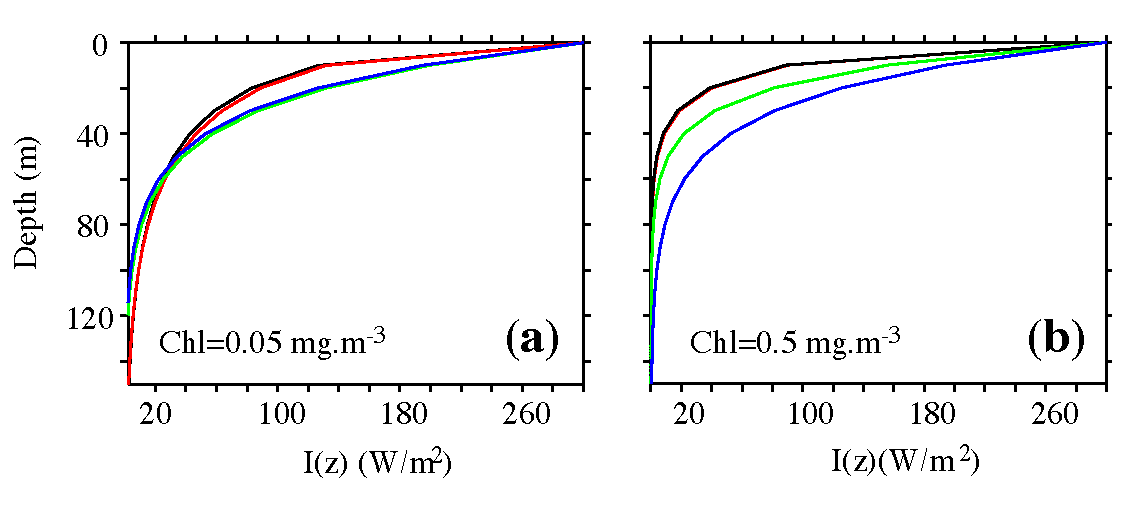
\includegraphics[width=1.0\textwidth]{Fig_TRA_Irradiance}
\caption{ 	 \label{Fig_traqsr_irradiance}
Penetration profile of the downward solar irradiance calculated by four models. 
Two waveband chlorophyll-independent formulation (blue), a chlorophyll-dependent 
monochromatic formulation (green), 4 waveband RGB formulation (red), 
61 waveband Morel (1988) formulation (black) for a chlorophyll concentration of 
(a) Chl=0.05 mg/m$^3$ and (b) Chl=0.5 mg/m$^3$. From \citet{Lengaigne_al_CD07}.}
\end{center}   \end{figure}
%>>>>>>>>>>>>>>>>>>>>>>>>>>>>

% -------------------------------------------------------------------------------------------------------------
%        Bottom Boundary Condition
% -------------------------------------------------------------------------------------------------------------
\subsection   [Bottom Boundary Condition (\textit{trabbc})]
			{Bottom Boundary Condition (\mdl{trabbc})}
\label{TRA_bbc}
%--------------------------------------------nambbc--------------------------------------------------------
\namdisplay{nambbc}
%--------------------------------------------------------------------------------------------------------------
%>>>>>>>>>>>>>>>>>>>>>>>>>>>>
\begin{figure}[!t] 	  \begin{center}
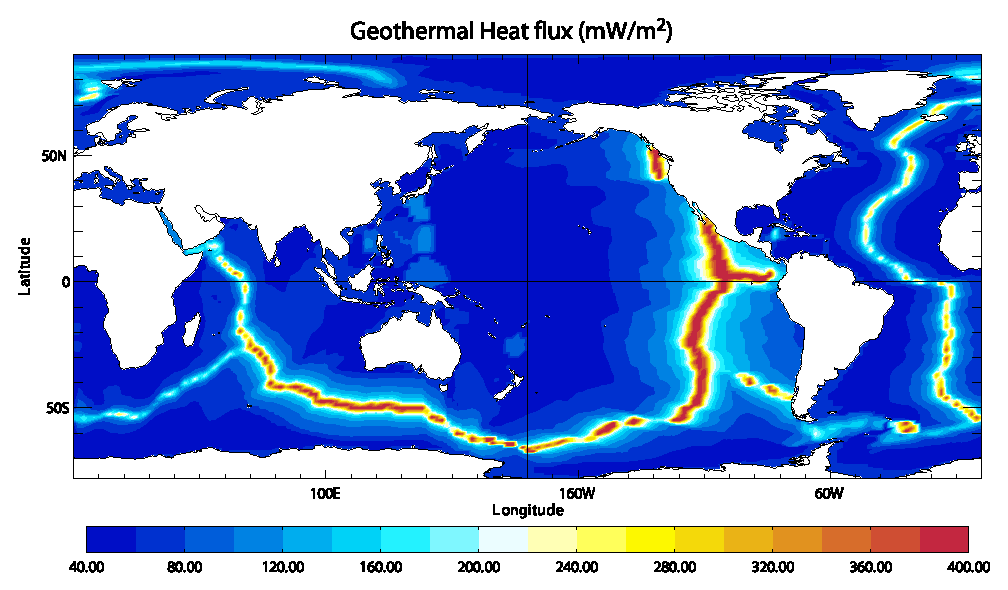
\includegraphics[width=1.0\textwidth]{Fig_TRA_geoth}
\caption{ 	\label{Fig_geothermal}
Geothermal Heat flux (in $mW.m^{-2}$) used by \cite{Emile-Geay_Madec_OS09}.
It is inferred from the age of the sea floor and the formulae of \citet{Stein_Stein_Nat92}.}
\end{center}   \end{figure}
%>>>>>>>>>>>>>>>>>>>>>>>>>>>>

Usually it is assumed that there is no exchange of heat or salt through 
the ocean bottom, $i.e.$ a no flux boundary condition is applied on active 
tracers at the bottom. This is the default option in \NEMO, and it is 
implemented using the masking technique. However, there is a 
non-zero heat flux across the seafloor that is associated with solid 
earth cooling. This flux is weak compared to surface fluxes (a mean 
global value of $\sim0.1\;W/m^2$ \citep{Stein_Stein_Nat92}), but it warms 
systematically the ocean and acts on the densest water masses. 
Taking this flux into account in a global ocean model increases
the deepest overturning cell ($i.e.$ the one associated with the Antarctic 
Bottom Water) by a few Sverdrups  \citep{Emile-Geay_Madec_OS09}. 

Options are defined through the  \ngn{namtra\_bbc} namelist variables.
The presence of geothermal heating is controlled by setting the namelist 
parameter  \np{ln\_trabbc} to true. Then, when \np{nn\_geoflx} is set to 1, 
a constant geothermal heating is introduced whose value is given by the 
\np{nn\_geoflx\_cst}, which is also a namelist parameter. 
When  \np{nn\_geoflx} is set to 2, a spatially varying geothermal heat flux is 
introduced which is provided in the \ifile{geothermal\_heating} NetCDF file 
(Fig.\ref{Fig_geothermal}) \citep{Emile-Geay_Madec_OS09}.

% ================================================================
% Bottom Boundary Layer
% ================================================================
\section  [Bottom Boundary Layer (\mdl{trabbl} - \key{trabbl})]
		{Bottom Boundary Layer (\mdl{trabbl} - \key{trabbl})}
\label{TRA_bbl}
%--------------------------------------------nambbl---------------------------------------------------------
\namdisplay{nambbl}
%--------------------------------------------------------------------------------------------------------------

Options are defined through the  \ngn{nambbl} namelist variables.
In a $z$-coordinate configuration, the bottom topography is represented by a 
series of discrete steps. This is not adequate to represent gravity driven 
downslope flows. Such flows arise either downstream of sills such as the Strait of 
Gibraltar or Denmark Strait, where dense water formed in marginal seas flows 
into a basin filled with less dense water, or along the continental slope when dense 
water masses are formed on a continental shelf. The amount of entrainment 
that occurs in these gravity plumes is critical in determining the density 
and volume flux of the densest waters of the ocean, such as Antarctic Bottom Water, 
or North Atlantic Deep Water. $z$-coordinate models tend to overestimate the 
entrainment, because the gravity flow is mixed vertically by convection 
as it goes ''downstairs'' following the step topography, sometimes over a thickness 
much larger than the thickness of the observed gravity plume. A similar problem 
occurs in the $s$-coordinate when the thickness of the bottom level varies rapidly 
downstream of a sill \citep{Willebrand_al_PO01}, and the thickness 
of the plume is not resolved. 

The idea of the bottom boundary layer (BBL) parameterisation, first introduced by 
\citet{Beckmann_Doscher1997}, is to allow a direct communication between 
two adjacent bottom cells at different levels, whenever the densest water is 
located above the less dense water. The communication can be by a diffusive flux
(diffusive BBL), an advective flux (advective BBL), or both. In the current 
implementation of the BBL, only the tracers are modified, not the velocities. 
Furthermore, it only connects ocean bottom cells, and therefore does not include 
all the improvements introduced by \citet{Campin_Goosse_Tel99}.

% -------------------------------------------------------------------------------------------------------------
%        Diffusive BBL
% -------------------------------------------------------------------------------------------------------------
\subsection{Diffusive Bottom Boundary layer (\np{nn\_bbl\_ldf}=1)}
\label{TRA_bbl_diff}

When applying sigma-diffusion (\key{trabbl} defined and \np{nn\_bbl\_ldf} set to 1), 
the diffusive flux between two adjacent cells at the ocean floor is given by 
\begin{equation} \label{Eq_tra_bbl_diff}
{\rm {\bf F}}_\sigma=A_l^\sigma \; \nabla_\sigma T
\end{equation} 
with $\nabla_\sigma$ the lateral gradient operator taken between bottom cells, 
and  $A_l^\sigma$ the lateral diffusivity in the BBL. Following \citet{Beckmann_Doscher1997}, 
the latter is prescribed with a spatial dependence, $i.e.$ in the conditional form
\begin{equation} \label{Eq_tra_bbl_coef}
A_l^\sigma (i,j,t)=\left\{ {\begin{array}{l}
 A_{bbl}  \quad \quad   \mbox{if}  \quad   \nabla_\sigma \rho  \cdot  \nabla H<0 \\ 
 \\
 0\quad \quad \;\,\mbox{otherwise} \\ 
 \end{array}} \right.
\end{equation} 
where $A_{bbl}$ is the BBL diffusivity coefficient, given by the namelist 
parameter \np{rn\_ahtbbl} and usually set to a value much larger 
than the one used for lateral mixing in the open ocean. The constraint in \eqref{Eq_tra_bbl_coef} 
implies that sigma-like diffusion only occurs when the density above the sea floor, at the top of 
the slope, is larger than in the deeper ocean (see green arrow in Fig.\ref{Fig_bbl}). 
In practice, this constraint is applied separately in the two horizontal directions, 
and the density gradient in \eqref{Eq_tra_bbl_coef} is evaluated with the log gradient formulation: 
\begin{equation} \label{Eq_tra_bbl_Drho}
	\nabla_\sigma \rho / \rho = \alpha \,\nabla_\sigma T + \beta   \,\nabla_\sigma S
\end{equation} 
where $\rho$, $\alpha$ and $\beta$ are functions of $\overline{T}^\sigma$, 
$\overline{S}^\sigma$ and $\overline{H}^\sigma$, the along bottom mean temperature, 
salinity and depth, respectively.

% -------------------------------------------------------------------------------------------------------------
%        Advective BBL
% -------------------------------------------------------------------------------------------------------------
\subsection   {Advective Bottom Boundary Layer  (\np{nn\_bbl\_adv}= 1 or 2)}
\label{TRA_bbl_adv}

\sgacomment{"downsloping flow" has been replaced by "downslope flow" in the following
if this is not what is meant then "downwards sloping flow" is also a possibility"}

%>>>>>>>>>>>>>>>>>>>>>>>>>>>>
\begin{figure}[!t] 	\begin{center}
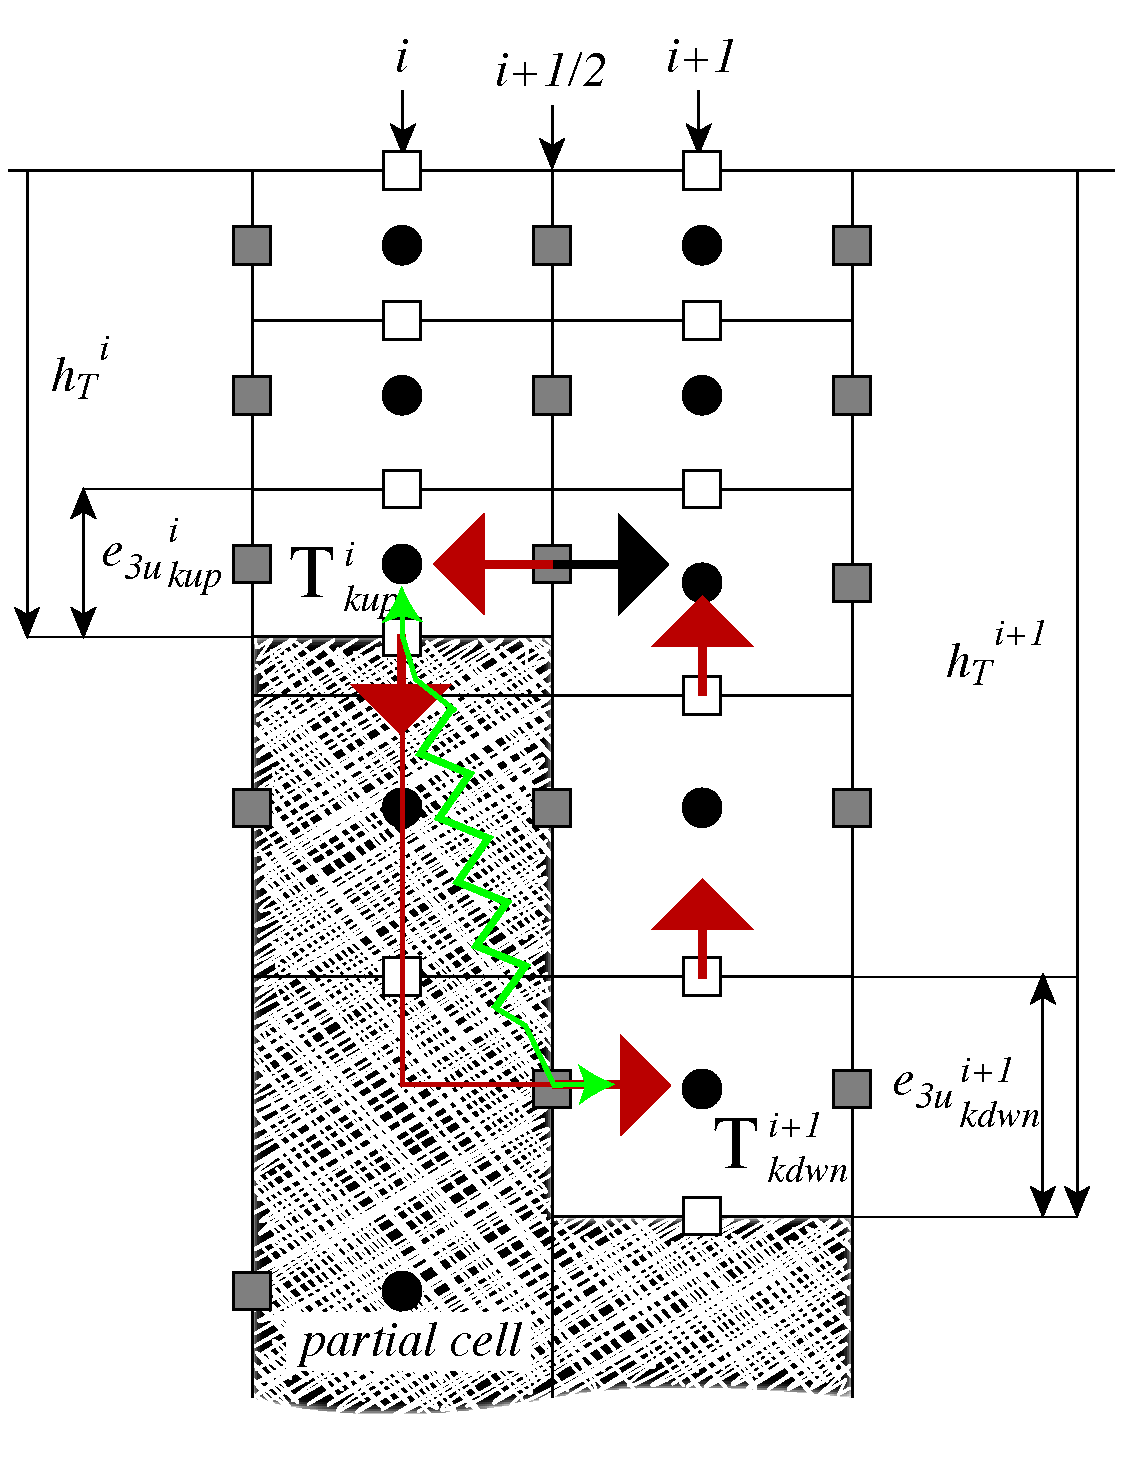
\includegraphics[width=0.7\textwidth]{Fig_BBL_adv}
\caption{ 	\label{Fig_bbl}  
Advective/diffusive Bottom Boundary Layer. The BBL parameterisation is 
activated when $\rho^i_{kup}$ is larger than $\rho^{i+1}_{kdnw}$. 
Red arrows indicate the additional overturning circulation due to the advective BBL. 
The transport of the downslope flow is defined either as the transport of the bottom 
ocean cell (black arrow), or as a function of the along slope density gradient. 
The green arrow indicates the diffusive BBL flux directly connecting $kup$ and $kdwn$
ocean bottom cells.
connection}
\end{center}   \end{figure}
%>>>>>>>>>>>>>>>>>>>>>>>>>>>>


%!!      nn_bbl_adv = 1   use of the ocean velocity as bbl velocity
%!!      nn_bbl_adv = 2   follow Campin and Goosse (1999) implentation
%!!        i.e. transport proportional to the along-slope density gradient

%%%gmcomment   :  this section has to be really written

When applying an advective BBL (\np{nn\_bbl\_adv} = 1 or 2), an overturning 
circulation is added which connects two adjacent bottom grid-points only if dense 
water overlies less dense water on the slope. The density difference causes dense 
water to move down the slope. 

\np{nn\_bbl\_adv} = 1 : the downslope velocity is chosen to be the Eulerian
ocean velocity just above the topographic step (see black arrow in Fig.\ref{Fig_bbl}) 
\citep{Beckmann_Doscher1997}. It is a \textit{conditional advection}, that is, advection
is allowed only if dense water overlies less dense water on the slope ($i.e.$ 
$\nabla_\sigma \rho  \cdot  \nabla H<0$) and if the velocity is directed towards 
greater depth ($i.e.$ $\vect{U}  \cdot  \nabla H>0$).

\np{nn\_bbl\_adv} = 2 : the downslope velocity is chosen to be proportional to $\Delta \rho$,
the density difference between the higher cell and lower cell densities \citep{Campin_Goosse_Tel99}.
The advection is allowed only  if dense water overlies less dense water on the slope ($i.e.$ 
$\nabla_\sigma \rho  \cdot  \nabla H<0$). For example, the resulting transport of the 
downslope flow, here in the $i$-direction (Fig.\ref{Fig_bbl}), is simply given by the 
following expression:
\begin{equation} \label{Eq_bbl_Utr}
 u^{tr}_{bbl} = \gamma \, g \frac{\Delta \rho}{\rho_o}  e_{1u} \; min \left( {e_{3u}}_{kup},{e_{3u}}_{kdwn} \right)
\end{equation}
where $\gamma$, expressed in seconds, is the coefficient of proportionality 
provided as \np{rn\_gambbl}, a namelist parameter, and \textit{kup} and \textit{kdwn} 
are the vertical index of the higher and lower cells, respectively.
The parameter $\gamma$ should take a different value for each bathymetric 
step, but for simplicity, and because no direct estimation of this parameter is 
available, a uniform value has been assumed. The possible values for $\gamma$ 
range between 1 and $10~s$ \citep{Campin_Goosse_Tel99}.  

Scalar properties are advected by this additional transport $( u^{tr}_{bbl}, v^{tr}_{bbl} )$ 
using the upwind scheme. Such a diffusive advective scheme has been chosen 
to mimic the entrainment between the downslope plume and the surrounding 
water at intermediate depths. The entrainment is replaced by the vertical mixing 
implicit in the advection scheme. Let us consider as an example the 
case displayed in Fig.\ref{Fig_bbl} where the density at level $(i,kup)$ is 
larger than the one at level $(i,kdwn)$. The advective BBL scheme
modifies the tracer time tendency of the ocean cells near the 
topographic step by the downslope flow \eqref{Eq_bbl_dw}, 
the horizontal \eqref{Eq_bbl_hor}  and the upward \eqref{Eq_bbl_up} 
return flows as follows: 
\begin{align} 
\partial_t T^{do}_{kdw} &\equiv \partial_t T^{do}_{kdw}
                                     +  \frac{u^{tr}_{bbl}}{{b_t}^{do}_{kdw}}  \left( T^{sh}_{kup} - T^{do}_{kdw} \right)  \label{Eq_bbl_dw} \\
%
\partial_t T^{sh}_{kup} &\equiv \partial_t T^{sh}_{kup} 
				   + \frac{u^{tr}_{bbl}}{{b_t}^{sh}_{kup}}   \left( T^{do}_{kup} - T^{sh}_{kup} \right)   \label{Eq_bbl_hor} \\
%
\intertext{and for $k =kdw-1,\;..., \; kup$ :} 
%
\partial_t T^{do}_{k} &\equiv \partial_t S^{do}_{k}
				   + \frac{u^{tr}_{bbl}}{{b_t}^{do}_{k}}   \left( T^{do}_{k+1} - T^{sh}_{k} \right)   \label{Eq_bbl_up}
\end{align}
where $b_t$ is the $T$-cell volume. 

Note that the BBL transport, $( u^{tr}_{bbl}, v^{tr}_{bbl} )$, is available in 
the model outputs. It has to be used to compute the effective velocity 
as well as the effective overturning circulation.

% ================================================================
% Tracer damping
% ================================================================
\section  [Tracer damping (\textit{tradmp})]
		{Tracer damping (\mdl{tradmp})}
\label{TRA_dmp}
%--------------------------------------------namtra_dmp-------------------------------------------------
\namdisplay{namtra_dmp}
%--------------------------------------------------------------------------------------------------------------

In some applications it can be useful to add a Newtonian damping term 
into the temperature and salinity equations:
\begin{equation} \label{Eq_tra_dmp}
\begin{split}
 \frac{\partial T}{\partial t}=\;\cdots \;-\gamma \,\left( {T-T_o } \right)  \\
 \frac{\partial S}{\partial t}=\;\cdots \;-\gamma \,\left( {S-S_o } \right) 
 \end{split}
 \end{equation} 
where $\gamma$ is the inverse of a time scale, and $T_o$ and $S_o$ 
are given temperature and salinity fields (usually a climatology). 
Options are defined through the  \ngn{namtra\_dmp} namelist variables.
The restoring term is added when the namelist parameter \np{ln\_tradmp} is set to true. 
It also requires that both \np{ln\_tsd\_init} and \np{ln\_tsd\_tradmp} are set to true
in \textit{namtsd} namelist as well as \np{sn\_tem} and \np{sn\_sal} structures are 
correctly set  ($i.e.$ that $T_o$ and $S_o$ are provided in input files and read 
using \mdl{fldread}, see \S\ref{SBC_fldread}). 
The restoring coefficient $\gamma$ is a three-dimensional array read in during the \rou{tra\_dmp\_init} routine. The file name is specified by the namelist variable \np{cn\_resto}. The DMP\_TOOLS tool is provided to allow users to generate the netcdf file.

The two main cases in which \eqref{Eq_tra_dmp} is used are \textit{(a)} 
the specification of the boundary conditions along artificial walls of a 
limited domain basin and \textit{(b)} the computation of the velocity 
field associated with a given $T$-$S$ field (for example to build the 
initial state of a prognostic simulation, or to use the resulting velocity 
field for a passive tracer study). The first case applies to regional 
models that have artificial walls instead of open boundaries. 
In the vicinity of these walls, $\gamma$ takes large values (equivalent to 
a time scale of a few days) whereas it is zero in the interior of the 
model domain. The second case corresponds to the use of the robust 
diagnostic method \citep{Sarmiento1982}. It allows us to find the velocity 
field consistent with the model dynamics whilst having a $T$, $S$ field 
close to a given climatological field ($T_o$, $S_o$). 

The robust diagnostic method is very efficient in preventing temperature 
drift in intermediate waters but it produces artificial sources of heat and salt 
within the ocean. It also has undesirable effects on the ocean convection. 
It tends to prevent deep convection and subsequent deep-water formation, 
by stabilising the water column too much.

The namelist parameter \np{nn\_zdmp} sets whether the damping should be applied in the whole water column or only below the mixed layer (defined either on a density or $S_o$ criterion). It is common to set the damping to zero in the mixed layer as the adjustment time scale is short here \citep{Madec_al_JPO96}.

\subsection[DMP\_TOOLS]{Generating resto.nc using DMP\_TOOLS}

DMP\_TOOLS can be used to generate a netcdf file containing the restoration coefficient $\gamma$. 
Note that in order to maintain bit comparison with previous NEMO versions DMP\_TOOLS must be compiled 
and run on the same machine as the NEMO model. A mesh\_mask.nc file for the model configuration is required as an input. 
This can be generated by carrying out a short model run with the namelist parameter \np{nn\_msh} set to 1. 
The namelist parameter \np{ln\_tradmp} will also need to be set to .false. for this to work. 
The \nl{nam\_dmp\_create} namelist in the DMP\_TOOLS directory is used to specify options for the restoration coefficient.

%--------------------------------------------nam_dmp_create-------------------------------------------------
\namdisplay{nam_dmp_create}
%-------------------------------------------------------------------------------------------------------

\np{cp\_cfg}, \np{cp\_cpz}, \np{jp\_cfg} and \np{jperio} specify the model configuration being used and should be the same as specified in \nl{namcfg}. The variable \nl{lzoom} is used to specify that the damping is being used as in case \textit{a} above to provide boundary conditions to a zoom configuration. In the case of the arctic or antarctic zoom configurations this includes some specific treatment. Otherwise damping is applied to the 6 grid points along the ocean boundaries. The open boundaries are specified by the variables \np{lzoom\_n}, \np{lzoom\_e}, \np{lzoom\_s}, \np{lzoom\_w} in the \nl{nam\_zoom\_dmp} name list.

The remaining switch namelist variables determine the spatial variation of the restoration coefficient in non-zoom configurations. 
\np{ln\_full\_field} specifies that newtonian damping should be applied to the whole model domain. 
\np{ln\_med\_red\_seas} specifies grid specific restoration coefficients in the Mediterranean Sea 
for the ORCA4, ORCA2 and ORCA05 configurations. 
If \np{ln\_old\_31\_lev\_code} is set then the depth variation of the coeffients will be specified as 
a function of the model number. This option is included to allow backwards compatability of the ORCA2 reference 
configurations with previous model versions. 
\np{ln\_coast} specifies that the restoration coefficient should be reduced near to coastlines. 
This option only has an effect if \np{ln\_full\_field} is true. 
\np{ln\_zero\_top\_layer} specifies that the restoration coefficient should be zero in the surface layer. 
Finally \np{ln\_custom} specifies that the custom module will be called. 
This module is contained in the file custom.F90 and can be edited by users. For example damping could be applied in a specific region.

The restoration coefficient can be set to zero in equatorial regions by specifying a positive value of \np{nn\_hdmp}. 
Equatorward of this latitude the restoration coefficient will be zero with a smooth transition to 
the full values of a 10\deg latitud band. 
This is often used because of the short adjustment time scale in the equatorial region 
\citep{Reverdin1991, Fujio1991, Marti_PhD92}. The time scale associated with the damping depends on the depth as a 
hyperbolic tangent, with \np{rn\_surf} as surface value, \np{rn\_bot} as bottom value and a transition depth of \np{rn\_dep}.  

% ================================================================
% Tracer time evolution
% ================================================================
\section  [Tracer time evolution (\textit{tranxt})]
		{Tracer time evolution (\mdl{tranxt})}
\label{TRA_nxt}
%--------------------------------------------namdom-----------------------------------------------------
\namdisplay{namdom}
%--------------------------------------------------------------------------------------------------------------

Options are defined through the  \ngn{namdom} namelist variables.
The general framework for tracer time stepping is a modified leap-frog scheme 
\citep{Leclair_Madec_OM09}, $i.e.$ a three level centred time scheme associated 
with a Asselin time filter (cf. \S\ref{STP_mLF}):
\begin{equation} \label{Eq_tra_nxt}
\begin{aligned}
(e_{3t}T)^{t+\rdt} &= (e_{3t}T)_f^{t-\rdt} &+ 2 \, \rdt  \,e_{3t}^t\ \text{RHS}^t &	\\
\\
(e_{3t}T)_f^t  \;\ \quad &= (e_{3t}T)^t \;\quad 
                                    &+\gamma \,\left[ {(e_{3t}T)_f^{t-\rdt} -2(e_{3t}T)^t+(e_{3t}T)^{t+\rdt}} \right] &  \\
                                 & &- \gamma\,\rdt \, \left[ Q^{t+\rdt/2} -  Q^{t-\rdt/2} \right]  &                      
\end{aligned}
\end{equation} 
where RHS is the right hand side of the temperature equation, 
the subscript $f$ denotes filtered values, $\gamma$ is the Asselin coefficient,
and $S$ is the total forcing applied on $T$ ($i.e.$ fluxes plus content in mass exchanges). 
$\gamma$ is initialized as \np{rn\_atfp} (\textbf{namelist} parameter). 
Its default value is \np{rn\_atfp}=$10^{-3}$. Note that the forcing correction term in the filter
is not applied in linear free surface (\jp{lk\_vvl}=false) (see \S\ref{TRA_sbc}.
Not also that in constant volume case, the time stepping is performed on $T$, 
not on its content, $e_{3t}T$.

When the vertical mixing is solved implicitly, the update of the \textit{next} tracer 
fields is done in module \mdl{trazdf}. In this case only the swapping of arrays 
and the Asselin filtering is done in the \mdl{tranxt} module.

In order to prepare for the computation of the \textit{next} time step, 
a swap of tracer arrays is performed: $T^{t-\rdt} = T^t$ and $T^t = T_f$. 

% ================================================================
% Equation of State (eosbn2) 
% ================================================================
\section  [Equation of State (\textit{eosbn2}) ]
		{Equation of State (\mdl{eosbn2}) }
\label{TRA_eosbn2}
%--------------------------------------------nameos-----------------------------------------------------
\namdisplay{nameos}
%--------------------------------------------------------------------------------------------------------------

% -------------------------------------------------------------------------------------------------------------
%        Equation of State
% -------------------------------------------------------------------------------------------------------------
\subsection{Equation Of Seawater (\np{nn\_eos} = -1, 0, or 1)}
\label{TRA_eos}

The Equation Of Seawater (EOS) is an empirical nonlinear thermodynamic relationship 
linking seawater density, $\rho$, to a number of state variables, 
most typically temperature, salinity and pressure. 
Because density gradients control the pressure gradient force through the hydrostatic balance, 
the equation of state provides a fundamental bridge between the distribution of active tracers 
and the fluid dynamics. Nonlinearities of the EOS are of major importance, in particular 
influencing the circulation through determination of the static stability below the mixed layer, 
thus controlling rates of exchange between the atmosphere  and the ocean interior \citep{Roquet_JPO2015}. 
Therefore an accurate EOS based on either the 1980 equation of state (EOS-80, \cite{UNESCO1983}) 
or TEOS-10 \citep{TEOS10} standards should be used anytime a simulation of the real 
ocean circulation is attempted \citep{Roquet_JPO2015}. 
The use of TEOS-10 is highly recommended because 
\textit{(i)} it is the new official EOS, 
\textit{(ii)} it is more accurate, being based on an updated database of laboratory measurements, and 
\textit{(iii)} it uses Conservative Temperature and Absolute Salinity (instead of potential temperature 
and practical salinity for EOS-980, both variables being more suitable for use as model variables 
\citep{TEOS10, Graham_McDougall_JPO13}. 
EOS-80 is an obsolescent feature of the NEMO system, kept only for backward compatibility.
For process studies, it is often convenient to use an approximation of the EOS. To that purposed, 
a simplified EOS (S-EOS) inspired by \citet{Vallis06} is also available.

In the computer code, a density anomaly, $d_a= \rho / \rho_o - 1$, 
is computed, with $\rho_o$ a reference density. Called \textit{rau0} 
in the code, $\rho_o$ is set in \mdl{phycst} to a value of $1,026~Kg/m^3$. 
This is a sensible choice for the reference density used in a Boussinesq ocean 
climate model, as, with the exception of only a small percentage of the ocean, 
density in the World Ocean varies by no more than 2$\%$ from that value \citep{Gill1982}.

Options are defined through the  \ngn{nameos} namelist variables, and in particular \np{nn\_eos} 
which controls the EOS used (=-1 for TEOS10 ; =0 for EOS-80 ; =1 for S-EOS).
\begin{description}

\item[\np{nn\_eos}$=-1$] the polyTEOS10-bsq equation of seawater \citep{Roquet_OM2015} is used.  
The accuracy of this approximation is comparable to the TEOS-10 rational function approximation, 
but it is optimized for a boussinesq fluid and the polynomial expressions have simpler 
and more computationally efficient expressions for their derived quantities 
which make them more adapted for use in ocean models. 
Note that a slightly higher precision polynomial form is now used replacement of the TEOS-10 
rational function approximation for hydrographic data analysis  \citep{TEOS10}. 
A key point is that conservative state variables are used: 
Absolute Salinity (unit: g/kg, notation: $S_A$) and Conservative Temperature (unit: \degC, notation: $\Theta$).
The pressure in decibars is approximated by the depth in meters. 
With TEOS10, the specific heat capacity of sea water, $C_p$, is a constant. It is set to 
$C_p=3991.86795711963~J\,Kg^{-1}\,^{\circ}K^{-1}$, according to \citet{TEOS10}.

Choosing polyTEOS10-bsq implies that the state variables used by the model are 
$\Theta$ and $S_A$. In particular, the initial state deined by the user have to be given as 
\textit{Conservative} Temperature and \textit{Absolute} Salinity. 
In addition, setting \np{ln\_useCT} to \textit{true} convert the Conservative SST to potential SST 
prior to either computing the air-sea and ice-sea fluxes (forced mode) 
or sending the SST field to the atmosphere (coupled mode).

\item[\np{nn\_eos}$=0$] the polyEOS80-bsq equation of seawater is used.
It takes the same polynomial form as the polyTEOS10, but the coefficients have been optimized 
to accurately fit EOS80 (Roquet, personal comm.). The state variables used in both the EOS80 
and the ocean model are: 
the Practical Salinity ((unit: psu, notation: $S_p$)) and Potential Temperature (unit: $^{\circ}C$, notation: $\theta$).
The pressure in decibars is approximated by the depth in meters.  
With thsi EOS, the specific heat capacity of sea water, $C_p$, is a function of temperature, 
salinity and pressure \citep{UNESCO1983}. Nevertheless, a severe assumption is made in order to 
have a heat content ($C_p T_p$) which is conserved by the model: $C_p$ is set to a constant 
value, the TEOS10 value. 
 
\item[\np{nn\_eos}$=1$] a simplified EOS (S-EOS) inspired by \citet{Vallis06} is chosen, 
the coefficients of which has been optimized to fit the behavior of TEOS10 (Roquet, personal comm.) 
(see also \citet{Roquet_JPO2015}). It provides a simplistic linear representation of both 
cabbeling and thermobaricity effects which is enough for a proper treatment of the EOS 
in theoretical studies \citep{Roquet_JPO2015}.
With such an equation of state there is no longer a distinction between 
\textit{conservative} and \textit{potential} temperature, as well as between \textit{absolute} 
and \textit{practical} salinity.
S-EOS takes the following expression:
\begin{equation} \label{Eq_tra_S-EOS}
\begin{split}
  d_a(T,S,z)  =  ( & - a_0 \; ( 1 + 0.5 \; \lambda_1 \; T_a + \mu_1 \; z ) * T_a  \\
                                & + b_0 \; ( 1 - 0.5 \; \lambda_2 \; S_a - \mu_2 \; z ) * S_a  \\
                                & - \nu \; T_a \; S_a \;  ) \; / \; \rho_o                     \\
  with \ \  T_a = T-10  \; ;  & \;  S_a = S-35  \; ;\;  \rho_o = 1026~Kg/m^3
\end{split}
\end{equation} 
where the computer name of the coefficients as well as their standard value are given in \ref{Tab_SEOS}.
In fact, when choosing S-EOS, various approximation of EOS can be specified simply by changing 
the associated coefficients. 
Setting to zero the two thermobaric coefficients ($\mu_1$, $\mu_2$) remove thermobaric effect from S-EOS.
setting to zero the three cabbeling coefficients ($\lambda_1$, $\lambda_2$, $\nu$) remove cabbeling effect from S-EOS.
Keeping non-zero value to $a_0$ and $b_0$ provide a linear EOS function of T and S.

\end{description}


%>>>>>>>>>>>>>>>>>>>>>>>>>>>>
\begin{table}[!tb]
\begin{center} \begin{tabular}{|p{26pt}|p{72pt}|p{56pt}|p{136pt}|}
\hline
coeff.	& computer name   & S-EOS		&  description		                  \\ \hline
$a_0$       & \np{rn\_a0}     & 1.6550 $10^{-1}$ &  linear thermal expansion coeff. 	\\ \hline
$b_0$	      & \np{rn\_b0} 	   & 7.6554 $10^{-1}$ &  linear haline  expansion coeff. 	\\ \hline
$\lambda_1$	& \np{rn\_lambda1}& 5.9520 $10^{-2}$ &  cabbeling coeff. in $T^2$ 	      \\ \hline
$\lambda_2$	& \np{rn\_lambda2}& 5.4914 $10^{-4}$ &  cabbeling coeff. in $S^2$	 	   \\ \hline
$\nu$       & \np{rn\_nu}     & 2.4341 $10^{-3}$ &  cabbeling coeff. in $T \, S$ 	   \\ \hline
$\mu_1$     & \np{rn\_mu1} 	& 1.4970 $10^{-4}$ &  thermobaric coeff. in T    	   \\ \hline
$\mu_2$     & \np{rn\_mu2} 	& 1.1090 $10^{-5}$ &  thermobaric coeff. in S   	      \\ \hline
\end{tabular}
\caption{ \label{Tab_SEOS}
Standard value of S-EOS coefficients. }
\end{center}
\end{table}
%>>>>>>>>>>>>>>>>>>>>>>>>>>>>


% -------------------------------------------------------------------------------------------------------------
%        Brunt-V\"{a}is\"{a}l\"{a} Frequency
% -------------------------------------------------------------------------------------------------------------
\subsection{Brunt-V\"{a}is\"{a}l\"{a} Frequency (\np{nn\_eos} = 0, 1 or 2)}
\label{TRA_bn2}

An accurate computation of the ocean stability (i.e. of $N$, the brunt-V\"{a}is\"{a}l\"{a}
 frequency) is of paramount importance as determine the ocean stratification and 
 is used in several ocean parameterisations (namely TKE, GLS, Richardson number dependent 
 vertical diffusion, enhanced vertical diffusion, non-penetrative convection, tidal mixing 
 parameterisation, iso-neutral diffusion). In particular, $N^2$ has to be computed at the local pressure 
 (pressure in decibar being approximated by the depth in meters). The expression for $N^2$ 
 is given by: 
\begin{equation} \label{Eq_tra_bn2}
N^2 =	\frac{g}{e_{3w}} \left(   \beta \;\delta_{k+1/2}[S] - \alpha \;\delta_{k+1/2}[T]   \right)
\end{equation} 
where $(T,S) = (\Theta, S_A)$ for TEOS10, $= (\theta, S_p)$ for TEOS-80, or $=(T,S)$ for S-EOS, 
and, $\alpha$ and $\beta$ are the thermal and haline expansion coefficients. 
The coefficients are a polynomial function of temperature, salinity and depth which expression 
depends on the chosen EOS. They are computed through \textit{eos\_rab}, a \textsc{Fortran} 
function that can be found in \mdl{eosbn2}.

% -------------------------------------------------------------------------------------------------------------
%        Freezing Point of Seawater
% -------------------------------------------------------------------------------------------------------------
\subsection   [Freezing Point of Seawater]
			{Freezing Point of Seawater}
\label{TRA_fzp}

The freezing point of seawater is a function of salinity and pressure \citep{UNESCO1983}:
\begin{equation} \label{Eq_tra_eos_fzp}
   \begin{split}
T_f (S,p) = \left( -0.0575 + 1.710523 \;10^{-3} \, \sqrt{S} 
						     -  2.154996 \;10^{-4} \,S  \right) \ S    \\
               - 7.53\,10^{-3} \ \ p 
   \end{split}
\end{equation}

\eqref{Eq_tra_eos_fzp} is only used to compute the potential freezing point of 
sea water ($i.e.$ referenced to the surface $p=0$), thus the pressure dependent 
terms in \eqref{Eq_tra_eos_fzp} (last term) have been dropped. The freezing
point is computed through \textit{eos\_fzp}, a \textsc{Fortran} function that can be found 
in \mdl{eosbn2}.  

% ================================================================
% Horizontal Derivative in zps-coordinate 
% ================================================================
\section  [Horizontal Derivative in \textit{zps}-coordinate (\textit{zpshde})]
		{Horizontal Derivative in \textit{zps}-coordinate (\mdl{zpshde})}
\label{TRA_zpshde}

\gmcomment{STEVEN: to be consistent with earlier discussion of differencing and averaging operators, 
                   I've changed "derivative" to "difference" and "mean" to "average"}

With partial cells (\np{ln\_zps}=true) at bottom and top (\np{ln\_isfcav}=true), in general, tracers in horizontally 
adjacent cells live at different depths. Horizontal gradients of tracers are needed 
for horizontal diffusion (\mdl{traldf} module) and for the hydrostatic pressure 
gradient (\mdl{dynhpg} module) to be active. 
\gmcomment{STEVEN from gm : question: not sure of  what -to be active- means}

Before taking horizontal gradients between the tracers next to the bottom, a linear 
interpolation in the vertical is used to approximate the deeper tracer as if it actually 
lived at the depth of the shallower tracer point (Fig.~\ref{Fig_Partial_step_scheme}). 
For example, for temperature in the $i$-direction the needed interpolated 
temperature, $\widetilde{T}$, is:

%>>>>>>>>>>>>>>>>>>>>>>>>>>>>
\begin{figure}[!p] 	 \begin{center}
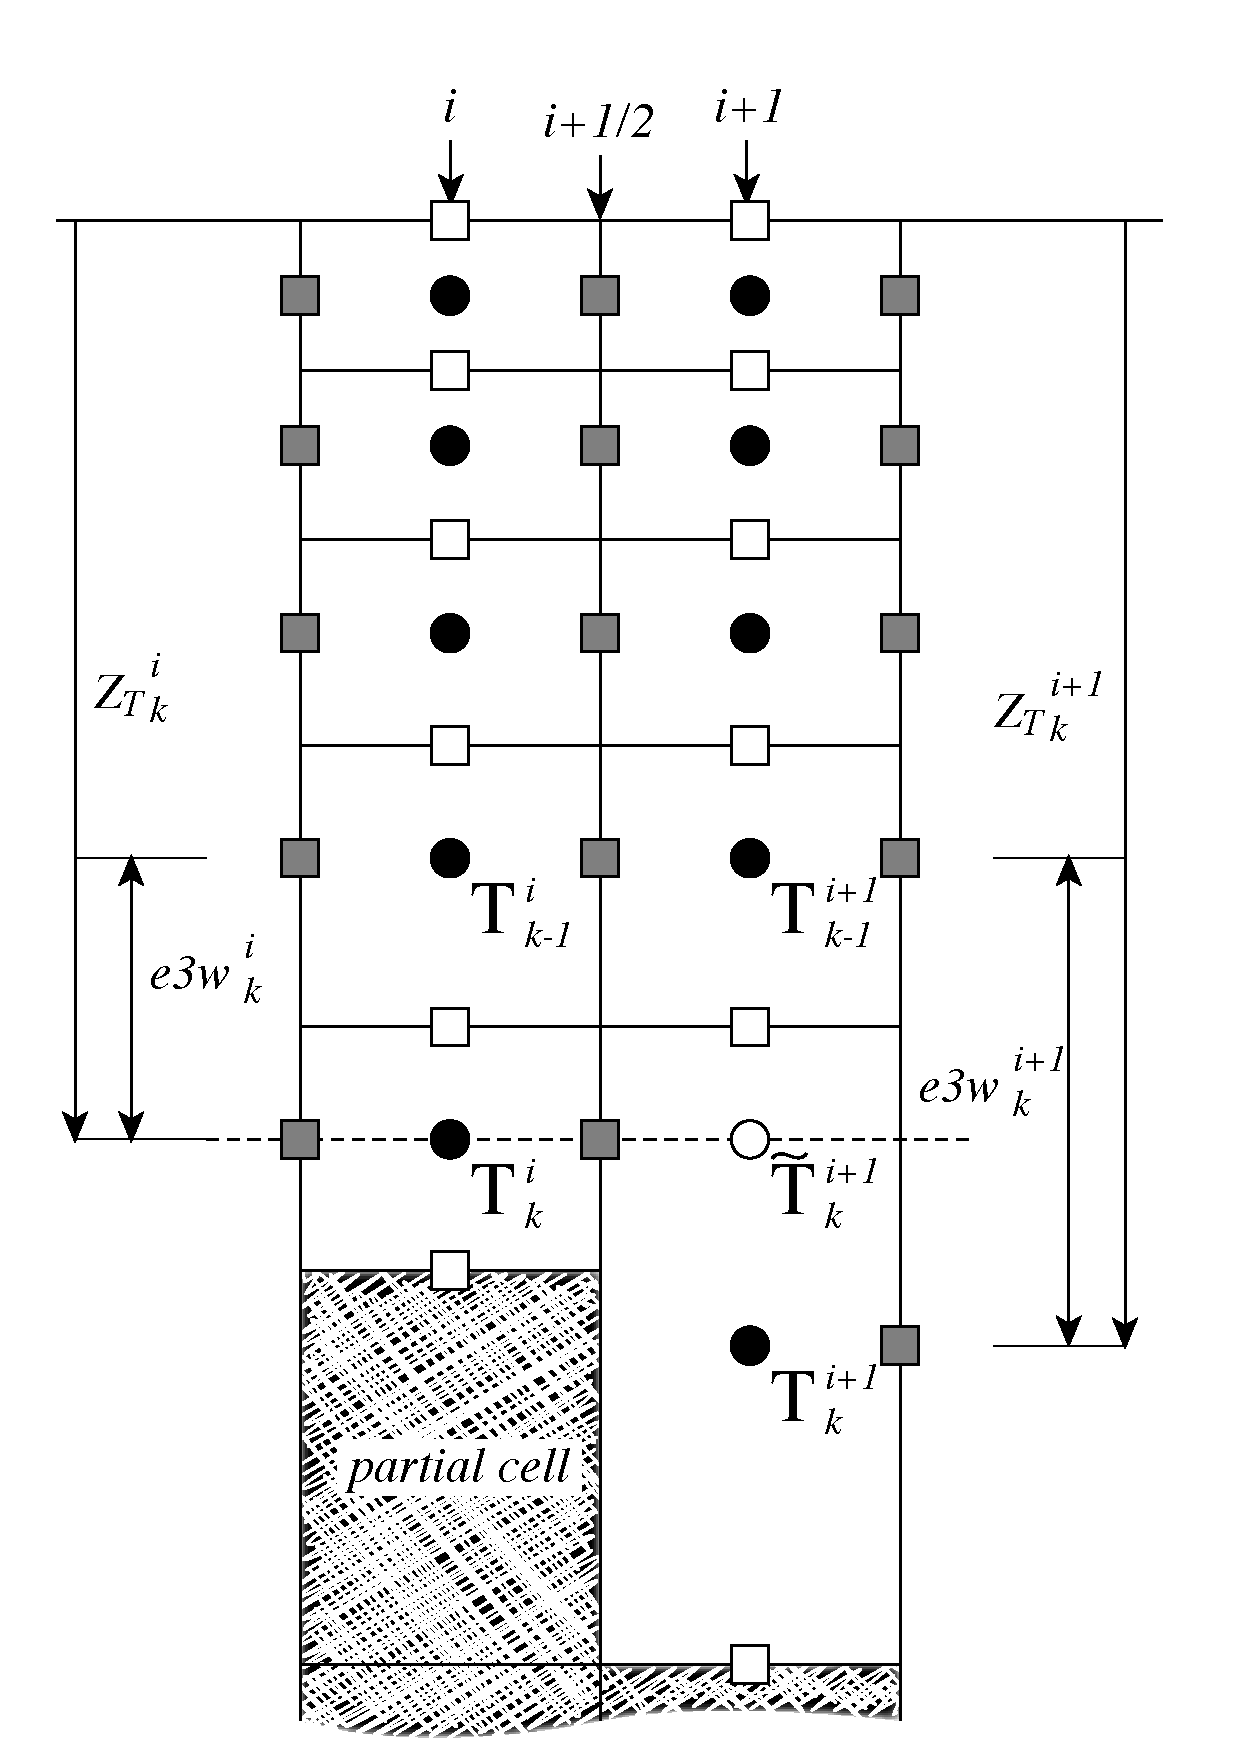
\includegraphics[width=0.9\textwidth]{Partial_step_scheme}
\caption{ 	\label{Fig_Partial_step_scheme} 
Discretisation of the horizontal difference and average of tracers in the $z$-partial 
step coordinate (\np{ln\_zps}=true) in the case $( e3w_k^{i+1} - e3w_k^i  )>0$. 
A linear interpolation is used to estimate $\widetilde{T}_k^{i+1}$, the tracer value 
at the depth of the shallower tracer point of the two adjacent bottom $T$-points. 
The horizontal difference is then given by: $\delta _{i+1/2} T_k=  \widetilde{T}_k^{\,i+1} -T_k^{\,i}$ 
and the average by: $\overline{T}_k^{\,i+1/2}= ( \widetilde{T}_k^{\,i+1/2} - T_k^{\,i} ) / 2$.  }
\end{center}   \end{figure}
%>>>>>>>>>>>>>>>>>>>>>>>>>>>>
\begin{equation*}
\widetilde{T}= \left\{  \begin{aligned}  
&T^{\,i+1}      -\frac{ \left( e_{3w}^{i+1} -e_{3w}^i \right)}{ e_{3w}^{i+1} }\;\delta _k T^{i+1}	
 								&& \quad\text{if  $\ e_{3w}^{i+1} \geq e_{3w}^i$   } 	\\
										\\
&T^{\,i} \ \ \ \,+\frac{ \left( e_{3w}^{i+1} -e_{3w}^i \right) }{e_{3w}^i       }\;\delta _k T^{i+1}
			 					&& \quad\text{if  $\ e_{3w}^{i+1}    <   e_{3w}^i$   } 
            \end{aligned}   \right.
\end{equation*}
and the resulting forms for the horizontal difference and the horizontal average 
value of $T$ at a $U$-point are: 
\begin{equation} \label{Eq_zps_hde}
\begin{aligned}
 \delta _{i+1/2} T= 	\begin{cases}
\ \ \ \widetilde {T}\quad\ -T^i	 	& \ \ \quad\quad\text{if  $\ e_{3w}^{i+1} \geq e_{3w}^i$ } \\
										\\
\ \ \ T^{\,i+1}-\widetilde{T}		& \ \ \quad\quad\text{if  $\ e_{3w}^{i+1}    <   e_{3w}^i$   } 
            		\end{cases}     \\
\\
\overline {T}^{\,i+1/2} \ = 	\begin{cases}
( \widetilde {T}\ \ \;\,-T^{\,i})	 / 2	& \;\ \ \quad\text{if  $\ e_{3w}^{i+1} \geq e_{3w}^i$ } \\
										\\
( T^{\,i+1}-\widetilde{T} ) / 2		& \;\ \ \quad\text{if  $\ e_{3w}^{i+1}    <   e_{3w}^i$   } 
            \end{cases}
\end{aligned}
\end{equation}

The computation of horizontal derivative of tracers as well as of density is 
performed once for all at each time step in \mdl{zpshde} module and stored 
in shared arrays to be used when needed. It has to be emphasized that the 
procedure used to compute the interpolated density, $\widetilde{\rho}$, is not 
the same as that used for $T$ and $S$. Instead of forming a linear approximation 
of density, we compute $\widetilde{\rho }$ from the interpolated values of $T$ 
and $S$, and the pressure at a $u$-point (in the equation of state pressure is 
approximated by depth, see \S\ref{TRA_eos} ) : 
\begin{equation} \label{Eq_zps_hde_rho}
\widetilde{\rho } = \rho ( {\widetilde{T},\widetilde {S},z_u }) 
\quad \text{where }\  z_u = \min \left( {z_T^{i+1} ,z_T^i } \right)
\end{equation} 

This is a much better approximation as the variation of $\rho$ with depth (and 
thus pressure) is highly non-linear with a true equation of state and thus is badly 
approximated with a linear interpolation. This approximation is used to compute 
both the horizontal pressure gradient (\S\ref{DYN_hpg}) and the slopes of neutral 
surfaces (\S\ref{LDF_slp})

Note that in almost all the advection schemes presented in this Chapter, both 
averaging and differencing operators appear. Yet \eqref{Eq_zps_hde} has not 
been used in these schemes: in contrast to diffusion and pressure gradient 
computations, no correction for partial steps is applied for advection. The main 
motivation is to preserve the domain averaged mean variance of the advected 
field when using the $2^{nd}$ order centred scheme. Sensitivity of the advection 
schemes to the way horizontal averages are performed in the vicinity of partial 
cells should be further investigated in the near future.
%%%
\gmcomment{gm :   this last remark has to be done}
%%%

If under ice shelf seas opened (\np{ln\_isfcav}=true), the partial cell properties 
at the top are computed in the same way as for the bottom. Some extra variables are, 
however, computed to reduce the flow generated at the top and bottom if $z*$ coordinates activated.
The extra variables calculated and used by \S\ref{DYN_hpg_isf} are:

$\bullet$ $\overline{T}_k^{\,i+1/2}$ as described in \eqref{Eq_zps_hde}

$\bullet$ $\delta _{i+1/2} Z_{T_k} = \widetilde {Z}^{\,i}_{T_k}-Z^{\,i}_{T_k}$ to compute 
the pressure gradient correction term used by \eqref{Eq_dynhpg_sco} in \S\ref{DYN_hpg_isf},
 with $\widetilde {Z}_{T_k}$ the depth of the point $\widetilde {T}_{k}$ in case of $z^*$ coordinates 
(this term = 0 in z-coordinates)
\end{document}
